\documentclass[a4paper,hidelinks,14pt]{extarticle}

\usepackage[utf8]{inputenc}
\usepackage[T2A]{fontenc}
\usepackage[english, russian]{babel}
\usepackage{amsmath}
\usepackage{amsfonts}
\usepackage{mathtools}
\usepackage{datetime}
\usepackage[pdftex]{graphicx}
\usepackage{indentfirst}
\usepackage{asymptote}
\usepackage{systeme}
\usepackage{listings}
\usepackage[usenames,dvipsnames]{color}	
\usepackage[font={small,it}]{caption}
\usepackage{gensymb}
\usepackage{hyperref}
\usepackage[framed,autolinebreaks,numbered,useliterate]{mcode}
\newcommand{\Span}{\text{Span}}
\newcommand{\Img}{\text{Im}}
\newcommand{\Ker}{\text{Ker}}
\hypersetup{
	colorlinks=true,
	linkcolor=blue,
	filecolor=magenta,      
	urlcolor=cyan,
}

\begin{document}
	\begin{titlepage}
		
		\setlength{\parindent}{0ex}
		
		\begin{center}
			\textsc{
				\vspace{1ex}
				Научно исследовательский университет ИТМО \\
				\vspace{0.5ex}
				Факультет систем управления и робототехники \\
				\vspace{0.5ex}
			}
		\end{center}
		
		\vspace{50mm}
		
		\begin{center}
			Отчет по лабораторной работе №5 \\
			Кластеризация и PageRank
		\end{center}
		
		\vspace{50mm}
		
		\begin{minipage}{.55\linewidth}
			Выполнил студент группы R3280
			
			\smallskip
			
			Преподаватель
		\end{minipage}
		\hfill
		\begin{minipage}{.4\linewidth}
			\begin{flushright}
				Мовчан И. Е.
				\\
				Перегудин А. А.
			\end{flushright}
		\end{minipage}
		
		\vfill
		\begin{center}
			Санкт-Петербург
			\\
			2024
		\end{center}
		
	\end{titlepage}
	
	\section{Кластеризация}
	\subsection{Выбор графа}
	Для начала выберем связаный граф, состоящий из 21 вершины. В нём каждая вершина представляет из себя человека, а ребро - отношение дружбы между соответствующими людьми (считаем, что если человек с кем-то дружит, то это происходит взаимно).
	\begin{figure}[h]
		\centering
		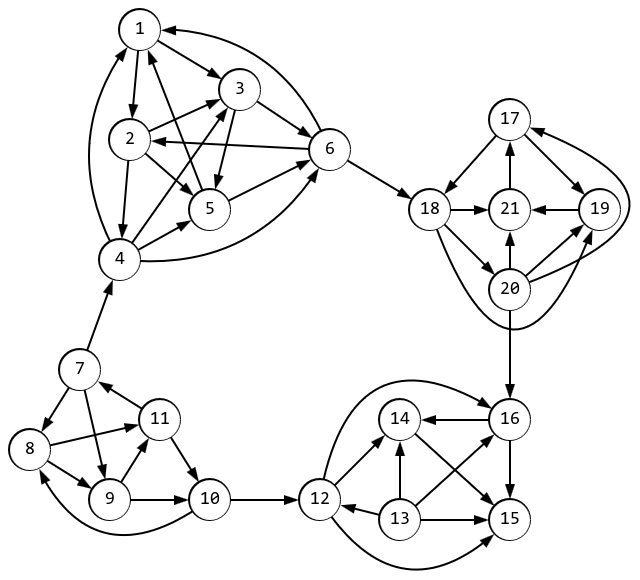
\includegraphics[scale=0.5]{./images/graph.png}
		\caption{Граф}
	\end{figure}
	
	Человеческий глаз запросто может выделить в нём 4 кластера (1-6, 7-10, 12-16, 17-21). Посмотрим, сможет ли это сделать компьютер? Для этого немного проанализируем наш граф.
	
	\subsection{Лапласиан, собственные числа и вектора}
	Итак, Лапласиан $L$ нашего графа будет иметь следующий вид:
	$$
	L = \begin{bsmallmatrix}
		5	&-1	&-1	&-1 &-1 &-1 &0	&0	&0	&0	&0	&0	&0	&0	&0	&0	&0	&0	&0	&0	&0\\
		-1&	5	&-1	&-1	&-1	&-1	&0	&0	&0	&0	&0	&0	&0	&0	&0	&0	&0	&0	&0	&0	&0\\
		-1&	-1	&5	&-1	&-1	&-1	&0	&0	&0	&0	&0	&0	&0	&0	&0	&0	&0	&0	&0	&0	&0\\
		-1&	-1	&-1	&6	&-1	&-1	&-1	&0	&0	&0	&0	&0	&0	&0	&0	&0	&0	&0	&0	&0	&0\\
		-1&	-1	&-1	&-1	&5	&-1	&0	&0	&0	&0	&0	&0	&0	&0	&0	&0	&0	&0	&0	&0	&0\\
		-1&	-1	&-1	&-1	&-1	&6	&0	&0	&0	&0	&0	&0	&0	&0	&0	&0	&0	&-1	&0	&0	&0\\
		0	&0	&0	&-1	&0	&0	&4	&-1	&-1	&0	&-1	&0	&0	&0	&0	&0	&0	&0	&0	&0	&0\\
		0	&0	&0	&0	&0	&0	&-1	&4	&-1	&-1	&-1	&0	&0	&0	&0	&0	&0	&0	&0	&0	&0\\
		0	&0	&0	&0	&0	&0	&-1	&-1	&4	&-1	&-1	&0	&0	&0	&0	&0	&0	&0	&0	&0	&0\\
		0	&0	&0	&0	&0	&0	&0	&-1	&-1	&4	&-1	&-1	&0	&0	&0	&0	&0	&0	&0	&0	&0\\
		0	&0	&0	&0	&0	&0	&-1	&-1	&-1	&-1	&4	&0	&0	&0	&0	&0	&0	&0	&0	&0	&0\\
		0	&0	&0	&0	&0	&0	&0	&0	&0	&-1	&0	&5	&-1	&-1	&-1	&-1	&0	&0	&0	&0	&0\\
		0	&0	&0	&0	&0	&0	&0	&0	&0	&0	&0	&-1	&4	&-1	&-1	&-1	&0	&0	&0	&0	&0\\
		0	&0	&0	&0	&0	&0	&0	&0	&0	&0	&0	&-1	&-1	&4	&-1	&-1	&0	&0	&0	&0	&0\\
		0	&0	&0	&0	&0	&0	&0	&0	&0	&0	&0	&-1	&-1	&-1	&4	&-1	&0	&0	&0	&0	&0\\
		0	&0	&0	&0	&0	&0	&0	&0	&0	&0	&0	&-1	&-1	&-1	&-1	&5	&0	&0	&0	&-1	&0\\
		0	&0	&0	&0	&0	&0	&0	&0	&0	&0	&0	&0	&0	&0	&0	&0	&4	&-1	&-1	&-1	&-1\\
		0	&0	&0	&0	&0	&-1	&0	&0	&0	&0	&0	&0	&0	&0	&0	&0	&-1	&5	&-1	&-1	&-1\\
		0	&0	&0	&0	&0	&0	&0	&0	&0	&0	&0	&0	&0	&0	&0	&0	&-1	&-1	&4	&-1	&-1\\
		0	&0	&0	&0	&0	&0	&0	&0	&0	&0	&0	&0	&0	&0	&0	&-1	&-1	&-1	&-1	&5	&-1\\
		0	&0	&0	&0	&0	&0	&0	&0	&0	&0	&0	&0	&0	&0	&0	&0	&-1	&-1	&-1	&-1	&4\\
	\end{bsmallmatrix}
	$$
	Выглядит довольно-таки устрашающе, но это только на первый взгляд.
	
	
	Собственные вектора будут иметь следующий вид:
	$$
	v_{1\phantom{1}}=\begin{bsmallmatrix}
		0.22\\
		0.22\\
		0.22\\
		0.22\\
		0.22\\
		0.22\\
		0.22\\
		0.22\\
		0.22\\
		0.22\\
		0.22\\
		0.22\\
		0.22\\
		0.22\\
		0.22\\
		0.22\\
		0.22\\
		0.22\\
		0.22\\
		0.22\\
		0.22\\
	\end{bsmallmatrix},
	v_{2\phantom{1}}=\begin{bsmallmatrix}
		-0.31\\
		-0.31\\
		-0.31\\
		-0.27\\
		-0.31\\
		-0.26\\
		-0.05\\
		0.03\\ 
		0.03\\ 
		0.1\\  
		0.03\\ 
		0.28\\ 
		0.32\\ 
		0.32\\ 
		0.32\\ 
		0.28\\ 
		0.02\\ 
		-0.03\\
		0.02\\ 
		0.07\\ 
		0.02\\
	\end{bsmallmatrix},
	v_{3\phantom{1}}=\begin{bsmallmatrix}
		 0.0\\  
		0.0\\  
		0.0\\  
		0.04\\ 
		0.0\\  
		-0.04\\
		0.28\\ 
		0.33\\  
		0.33\\  
		0.28\\  
		0.33\\  
		0.05\\  
		-0.0\\  
		-0.0\\  
		-0.0\\  
		-0.05\\ 
		-0.33\\ 
		-0.28\\
		-0.33\\ 
		-0.28\\ 
		-0.33\\ 
	\end{bsmallmatrix}
	v_{4\phantom{1}}=\begin{bsmallmatrix}
	-0.2\\   
	-0.2\\   
	-0.2\\   
	-0.14\\ 
	-0.2\\   
	-0.14\\
	0.19\\  
	0.26\\   
	0.26\\   
	0.17\\   
	0.26\\   
	-0.19\\  
	-0.27\\  
	-0.27\\  
	-0.27\\  
	-0.19\\ 
	0.26\\  
	0.18\\ 
	0.26\\  
	0.17\\  
	0.26\\  
	\end{bsmallmatrix},
		v_{5\phantom{1}}=\begin{bsmallmatrix}
		-0.06\\ 
		-0.06\\ 
		-0.06\\ 
		0.15\\ 
		-0.06\\ 
		-0.05\\ 
		0.65\\  
		0.01\\  
		0.01\\  
		-0.67\\ 
		0.01\\  
		-0.24\\ 
		0.1\\   
		0.1\\   
		0.1\\   
		0.07\\ 
		-0.0\\  
		-0.02\\
		-0.0\\  
		0.03\\  
		-0.0\\  
	\end{bsmallmatrix}
	$$
	$$
	v_{6\phantom{1}}=\begin{bsmallmatrix}
		  0.0\\ 
		0.0\\ 
		0.0\\ 
		-0.0\\
		0.0\\ 
		0.0\\ 
		-0.0\\ 
		0.08\\ 
		0.18\\ 
		-0.0\\
		-0.27\\
		-0.0\\
		0.64\\  
		-0.65\\ 
		-0.12\\ 
		0.13\\
		-0.14\\
		0.0\\
		-0.01\\
		0.13\\ 
		0.01\\ 
	\end{bsmallmatrix},
		v_{7\phantom{1}}=\begin{bsmallmatrix}
		 0.0\\   
		0.0\\   
		0.0\\   
		0.0\\  
		0.0\\   
		-0.0\\  
		-0.0\\  
		0.09\\  
		-0.26\\ 
		-0.0\\ 
		0.17\\ 
		-0.0\\ 
		0.37\\   
		0.1\\   
		-0.3\\  
		-0.17\\
		0.63\\ 
		-0.0\\ 
		-0.44\\
		-0.17\\ 
		-0.02\\ 
	\end{bsmallmatrix},
		v_{8\phantom{1}}=\begin{bsmallmatrix}
		0.0\\         
		0.0\\         
		0.0\\         
		-0.0\\       
		0.0\\         
		0.0\\        
		-0.0\\       
		-0.01\\      
		0.03\\      
		-0.0\\      
		-0.02\\     
		-0.0\\      
		0.05\\        
		0.07\\        
		0.05\\       
		-0.17\\    
		-0.31\\     
		0.0\\       
		-0.36\\    
		-0.17\\     
		0.84\\      
	\end{bsmallmatrix},
		v_{9\phantom{1}}=\begin{bsmallmatrix}
		0.0\\  
		-0.0\\ 
		-0.0\\ 
		0.0\\  
		-0.0\\ 
		-0.0\\ 
		0.0\\  
		0.42\\ 
		-0.02\\
		0.0\\  
		-0.4\\ 
		0.0\\  
		-0.32\\
		-0.25\\
		0.54\\ 
		0.03\\ 
		0.31\\ 
		-0.0\\ 
		-0.33\\
		0.03\\ 
		-0.01\\
	\end{bsmallmatrix},
		v_{10}=\begin{bsmallmatrix}
		0.0\\   -
		0.0\\   
		0.0\\   
		-0.0\\   
		-0.0\\  
		0.0\\   
		-0.0\\   
		-0.11\\ 
		-0.21\\
		-0.0\\   
		0.32\\  
		-0.0\\   
		-0.22\\
		-0.16\\
		-0.14\\ 
		0.52\\  
		-0.1\\  
		0.0\\   
		-0.45\\
		0.52\\  
		0.03\\
	\end{bsmallmatrix}
	$$
	$$
	v_{11}=\begin{bsmallmatrix}
		-0.0\\ 
		-0.0\\ 
		0.0\\  
		0.0\\  
		0.0\\  
		0.0\\  
		0.0\\  
		-0.64\\
		0.3\\  
		0.0\\  
		0.34\\ 
		0.0\\  
		0.01\\ 
		-0.31\\
		0.43\\ 
		-0.13\\
		0.24\\ 
		0.0\\  
		-0.1\\ 
		-0.13\\
		-0.01\\
	\end{bsmallmatrix},
	v_{12}=\begin{bsmallmatrix}
		  0.0\\   
		0.0\\   
		0.0\\    
		0.0\\    
		-0.0\\   
		-0.0\\   
		0.0\\    
		-0.22\\
		0.65\\   
		0.0\\    
		-0.43\\ 
		-0.0\\   
		-0.11\\ 
		0.3\\  
		-0.32\\ 
		0.13\\ 
		0.17\\  
		-0.0\\   
		-0.26\\ 
		0.13\\ 
		-0.04\\
	\end{bsmallmatrix},
	v_{13}=\begin{bsmallmatrix}
		  0.06\\     
		0.06\\     
		0.06\\      
		-0.26\\     
		0.06\\     
		0.08\\     
		-0.53\\     
		0.28\\  
		0.28\\     
		-0.36\\     
		0.28\\   
		-0.44\\    
		0.13\\   
		0.13\\    
		0.13\\   
		0.04\\   
		-0.05\\   
		0.1\\      
		-0.05\\  
		0.05\\   
		-0.05\\ 
	\end{bsmallmatrix},
	v_{14}=\begin{bsmallmatrix}
		   -0.13\\    
		-0.13\\    
		-0.13\\     
		-0.0\\     
		-0.13\\    
		0.42\\     
		0.08\\     
		-0.04\\ 
		-0.04\\    
		0.04\\     
		-0.04\\  
		0.05\\    
		0.02\\   
		0.02\\    
		0.02\\   
		-0.12\\  
		-0.21\\  
		0.77\\      
		-0.21\\ 
		-0.07\\  
		-0.21\\
	\end{bsmallmatrix},
	v_{15}=\begin{bsmallmatrix}
		      -0.64\\   
		   0.75\\    
		   0.04\\     
		   0.0\\      
		   -0.16\\   
		   0.0\\      
		   -0.0\\     
		   0.0\\  
		   -0.0\\    
		   -0.0\\     
		   0.0\\   
		   0.0\\     
		   0.0\\    
		   -0.0\\    
		   0.0\\    
		   -0.0\\  
		   0.0\\   
		   -0.0\\      
		   -0.0\\ 
		   0.0\\   
		   0.0\\ 
	\end{bsmallmatrix}
	$$
	$$
	v_{16}=\begin{bsmallmatrix}
		     0.39\\   
		0.39\\    
		-0.83\\    
		-0.0\\      
		0.06\\   
		-0.0\\      
		0.0\\      
		-0.0\\  
		0.0\\     
		-0.0\\     
		0.0\\    
		0.0\\      
		-0.0\\    
		-0.0\\    
		0.0\\     
		0.0\\   
		-0.0\\   
		-0.0\\      
		-0.0\\ 
		0.0\\    
		0.0\\  
	\end{bsmallmatrix},
	v_{17}=\begin{bsmallmatrix}
		     -0.44\\  
		-0.18\\   
		-0.23\\   
		-0.0\\      
		0.85\\   
		-0.0\\      
		0.0\\       
		-0.0\\  
		0.0\\      
		0.0\\      
		-0.0\\    
		-0.0\\      
		-0.0\\    
		0.0\\     
		-0.0\\     
		0.0\\    
		0.0\\    
		0.0\\       
		-0.0\\ 
		0.0\\     
		0.0\\   
	\end{bsmallmatrix},
	v_{18}=\begin{bsmallmatrix}
		         -0.02\\ 
		-0.02\\  
		-0.02\\  
		0.16\\      
		-0.02\\  
		-0.06\\     
		0.1\\        
		-0.13\\ 
		-0.13\\     
		0.46\\      
		-0.13\\   
		-0.67\\     
		0.2\\     
		0.2\\      
		0.2\\      
		-0.17\\   
		-0.06\\   
		-0.05\\      
		-0.06\\
		0.31\\     
		-0.06\\  
	\end{bsmallmatrix},
	v_{19}=\begin{bsmallmatrix}
		         -0.07\\
		-0.07\\ 
		-0.07\\ 
		0.14\\      
		-0.07\\ 
		0.21\\     
		-0.02\\       
		-0.03\\
		-0.03\\    
		0.16\\      
		-0.03\\  
		-0.35\\    
		-0.06\\    
		-0.06\\     
		-0.06\\     
		0.63\\   
		0.12\\   
		-0.0\\      
		0.12\\
		-0.56\\    
		0.12\\  
	\end{bsmallmatrix}
	$$
	$$
	v_{20}=\begin{bsmallmatrix}
		           0.2\\  
		0.2\\   
		0.2\\   
		-0.69\\      
		0.2\\   
		-0.33\\     
		0.3\\         
		-0.08\\
		-0.08\\    
		0.11\\       
		-0.08\\  
		-0.11\\    
		-0.0\\     
		-0.0\\      
		-0.0\\      
		0.13\\    
		-0.02\\   
		0.26\\       
		-0.02\\
		-0.16\\    
		-0.02\\ 
	\end{bsmallmatrix}, 
	v_{21}=\begin{bsmallmatrix}
		-0.04\\
		-0.04\\
		-0.04\\
		-0.5\\
		-0.04\\
		0.72\\
		0.18\\
		-0.04\\
		-0.04\\
		0.03\\
		-0.04\\
		-0.0\\
		0.01\\
		0.01\\
		0.01\\
		-0.07\\
		0.05\\
		-0.4\\
		0.05\\
		0.13\\
		0.05\\
	\end{bsmallmatrix}
	$$
	
	А вот собственные значения:
	$$
	\lambda_1=0,\,
	\lambda_2=0.26,\,
	\lambda_3=0.3,\,
	\lambda_4=0.61,\,
	\lambda_5=3.7
	$$
	$$
	\lambda_6=\lambda_7=\lambda_8=\lambda_9=\lambda_{10}=\lambda_{11}=\lambda_{12}=5,\,
	\lambda_{13}=5.13,\,
	\lambda_{14}=5.36
	$$
	$$
	\lambda_{15}=\lambda_{16}=6=\lambda_{17}=6,\,
	\lambda_{18}=6.31,\,
	\lambda_{19}=6.74,\,
	\lambda_{20}=7.11,\,
	\lambda_{21}=7.48
	$$
	
	\subsection{Кластеризация при $k=4$}
	Здесь k - количество кластеров, на которые мы хотим разбить наш граф. Начнём с оптимального значения (так как граф специально был разбит на 4 группы), чтобы было от чего отталкиваться.
	
	Итак, возьмём k самых малых собственных чисел. Для нас это $	\lambda_1=0,\, \lambda_2=0.26,\, \lambda_3=0.3,\, \lambda_4=0.61,$. Составим из соответствующих их векторов матрицу
	$$
	V = \begin{bmatrix}
		\vline & \vline & \vline & \vline \\
		v_1 & v_2 & v_3 & v_4 \\
		\vline & \vline & \vline & \vline \\
	\end{bmatrix}
	$$
	
	Получим:
	$$V=\begin{bsmallmatrix}
		0.22 & -0.31 & 0.0 &		-0.2 \\
		0.22 &		-0.31 & 0.0 &		-0.2 \\
		0.22&		-0.31 & 0.0 &		-0.2 \\
		0.22&		-0.27 & 0.04 &		-0.14 \\
		0.22&		-0.31 & 0.0 &		-0.2  \\
		0.22&		-0.26 & -0.04 &		-0.1 \\
		0.22&		-0.05 & 0.28 &		0.19 \\
		0.22&		0.03 & 0.33  &		0.26 \\
		0.22&		0.03 & 0.33  &		0.26 \\
		0.22&		0.1 & 0.28  &		0.17 \\
		0.22&		0.03 & 0.33  &		0.26 \\
		0.22&		0.28 & 0.05  &		-0.19  \\
		0.22&		0.32 & -0.0  &		-0.27  \\
		0.22&		0.32 & -0.0  &		-0.27  \\
		0.22&		0.32 & -0.0  &		-0.27  \\
		0.22&		0.28 & -0.05  &		-0.19 \\
		0.22&		0.02 & -0.33  &		0.26 \\
		0.22&		-0.03 & -0.28 &		0.18 \\
		0.22&		0.02 & -0.33  &		0.26 \\
		0.22&		0.07 & -0.28  &		0.17 \\
		0.22&		0.02 & -0.33  &		0.26 \\
	\end{bsmallmatrix}
	$$
	
	Далее, используя простой код в среде matlab, найдём разбиение на кластеры:
	\begin{lstlisting}
clusters = kmeans(V,k); % k = 4
	\end{lstlisting}
	
	Теперь в переменной $clusters$ хранятся числа от $1$ до $k$. Вершины попали в один и тот же кластер, если i число совпадает с j. Раскрасим наш граф, исходя из результата работы нашей программы:
	\begin{lstlisting}
2
2
2
2
2
2
3
3
3
3
3
1
1
1
1
1
4
4
4
4
4
	\end{lstlisting}
	\begin{figure}[h]
		\centering
		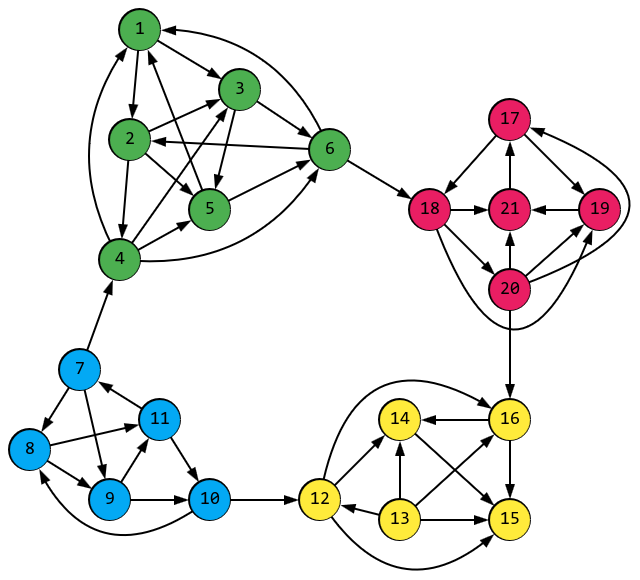
\includegraphics[scale=0.5]{./images/graph1.png}
		\caption{Кластеризация для k=4}
	\end{figure}
	
	Как видим, программа смогла очень точно определить нужные кластеры. Это успех!
	
	\subsection{Кластеризация для $k=2$}
	Посмотрим теперь на кластеризацию при различных значениях $k$.
	
	Пусть сначала $k=2$. Собственные значения системы будут следующими: $\lambda_1=0,\,
	\lambda_2=0.26$. Рассматриваемая же матрица, составленная из отвечающих этим числам векторов, примет вид:
		
		$$V=\begin{bsmallmatrix}
			0.22 & -0.31\\
			0.22 &		-0.31\\  
			0.22&		-0.31\\
			0.22&		-0.27\\ 
			0.22&		-0.31\\ 
			0.22&		-0.26\\ 
			0.22&		-0.05\\ 
			0.22&		0.03 \\
			0.22&		0.03 \\
			0.22&		0.1 \\
			0.22&		0.03 \\
			0.22&		0.28\\
			0.22&		0.32\\
			0.22&		0.32\\
			0.22&		0.32\\
			0.22&		0.28\\
			0.22&		0.02 \\
			0.22&		-0.03\\
			0.22&		0.02 \\
			0.22&		0.07 \\
			0.22&		0.02 \\
		\end{bsmallmatrix}
		$$
		
		Результатом работы программы будет:
		\begin{lstlisting}
2
2
2
2
2
2
2
2
2
2
2
2
2
2
2
2
1
1
1
1
1
		\end{lstlisting}
		
		Раскраска графа представлена на рисунке \ref{3}.
		\begin{figure}[h]
			\centering
			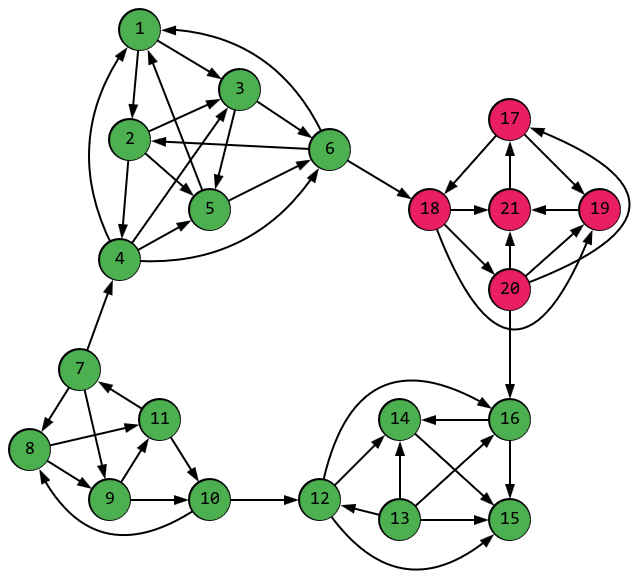
\includegraphics[scale=0.5]{./images/graph3.png}
			\caption{Кластеризация для k=2}
			\label{3}
		\end{figure}
		
		\subsection{Кластеризация для $k=6$}
		Первые k минимальные числа Лапласиана $L$ будут следующими: 
		$\lambda_1=0,\,
		\lambda_2=0.26,\,
		\lambda_3=0.3,\,
		\lambda_4=0.61,\,
		\lambda_5=3.7$
		
		Матрица, составленная из соответственных собственных векторов, в этом случае будет равна
		$$
		V=\begin{bsmallmatrix}
			0.22 & -0.31 & 0.0 &		   -0.2 & 		-0.06 & 		  0.0\\ 
			0.22 &		-0.31 & 0.0 &		-0.2 & 		-0.06 & 		0.0\\ 
			0.22&		-0.31 & 0.0 &		-0.2 & 		-0.06 & 		0.0\\ 
			0.22&		-0.27 & 0.04 &		-0.14 & 		0.15 & 		-0.0\\
			0.22&		-0.31 & 0.0 &		-0.2  & 		-0.06 & 		0.0\\ 
			0.22&		-0.26 & -0.04 &		-0.1 & 		-0.05 & 		0.0\\ 
			0.22&		-0.05 & 0.28 &		0.19 & 		0.65  & 		-0.0\\ 
			0.22&		0.03 & 0.33  &		0.26 & 		0.01 & 		0.08\\ 
			0.22&		0.03 & 0.33  &		0.26 & 		0.01 & 		0.18\\ 
			0.22&		0.1 & 0.28  &		0.17 & 		-0.67 & 		-0.0\\
			0.22&		0.03 & 0.33  &		0.26 & 		0.01 & 		-0.27\\
			0.22&		0.28 & 0.05  &		-0.19  & 		-0.24 & 		-0.0\\
			0.22&		0.32 & -0.0  &		-0.27  & 		0.1 & 		0.64\\  
			0.22&		0.32 & -0.0  &		-0.27  & 		0.1 & 		-0.65\\ 
			0.22&		0.32 & -0.0  &		-0.27  & 		0.1 & 		-0.12\\ 
			0.22&		0.28 & -0.05  &		-0.19 & 		0.07 & 		0.13\\
			0.22&		0.02 & -0.33  &		0.26 & 		-0.0 & 		-0.14\\
			0.22&		-0.03 & -0.28 &		0.18 & 		-0.0 & 		0.0\\
			0.22&		0.02 & -0.33  &		0.26 & 		-0.0 & 		-0.01\\
			0.22&		0.07 & -0.28  &		0.17 & 		0.03 & 		0.13\\ 
			0.22&		0.02 & -0.33  &		0.26 & 		-0.0 & 		0.01\\ 
		\end{bsmallmatrix}
		$$
		
		А вот результат работы кода:
		\begin{lstlisting}
6
6
6
1
6
6
4
4
4
4
4
3
5
5
5
3
2
2
2
2
2
		\end{lstlisting}
		
		Раскрашенный граф представлен на рисунке \ref{4}.
		\begin{figure}[h]
			\centering
			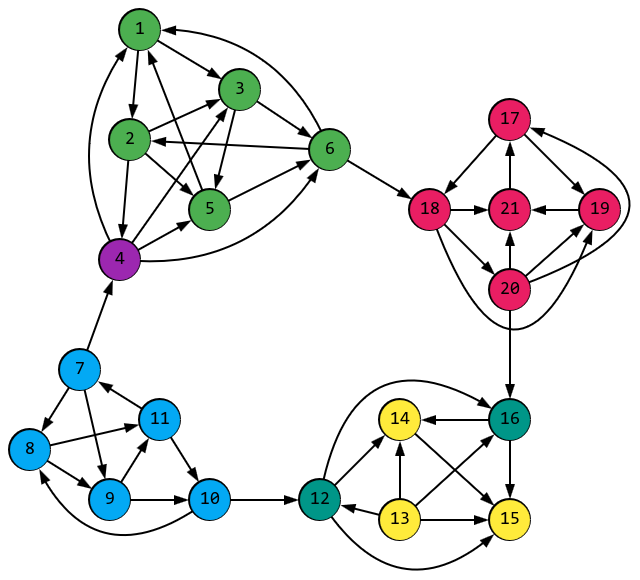
\includegraphics[scale=0.5]{./images/graph4.png}
			\caption{Кластеризация для k=6}
			\label{4}
		\end{figure}
		
		Видим, что как при уменьшении, так и при увеличении k теряется точность (при больших k, например, появляются отдельные островки одиночек, которые, как мы подсознательно понимаем, никакого отношения ни к одному из кластеров не имеют; при маленьких же происходит неуместное объединение в объёмные группы, что нам тоже не нравится).
	
	\subsection{Раскрытие магии}
	Давайте детально разберём метод k-means и поймём, что на самом деле за ним прячется довольно-таки простая математика.
	
	Итак, метод k-means основан на минимизации суммы квадратов расстояний элементов центроидов (неких центров масс). Сначала берутся k произвольных точек в пространстве - мы-то их и называем центроидами (вообще говоря, лучше брать либо сами рассматриваемые точки, либо использовать методы по оптимальному их расположению, ведь качество кластеризации в методе k-means напрямую зависит ещё и от того, как мы поставили исходные точки).
	
	Далее каждая точка примыкает к своему центроиду исходя из расстояния до каждого (выбирается минимальное). После для каждой из групп вычисляется новый центр, являющийся средним между значениями всех точек внутри рассматриваемого кластера.
	
	Процедура объединения в кластеры и поиска нового центроида для каждого продолжается до тех пор, пока мы не придём к стабильности (но обычно на число шагов ставится ограничение, оно и понятно - никто не хочет ждать тысячу лет, пока точки разобъёт на кластеры).
	
	Соответственно, качество кластеризации мы можем оценить по сумме расстояний внутри кластеров.
	
	Вот, вообще никакой магии - простая арифметика!
	
	\section{Google PageRank алгоритм}
	В задании попробуем применить алгоритм сортировки страниц, когда-то используемый компанией Google.
	
	\subsection{Выбор графа}
	
	Перед тем, как приступить к работе, необходимо выбрать ориентированный граф, каждая вершина которого по своей сути будет являться веб-страницей, а стрелка - ссылкой, позволяющей пользователю перейти с одной страницы на другую.
	
	\begin{figure}[h]
		\centering
		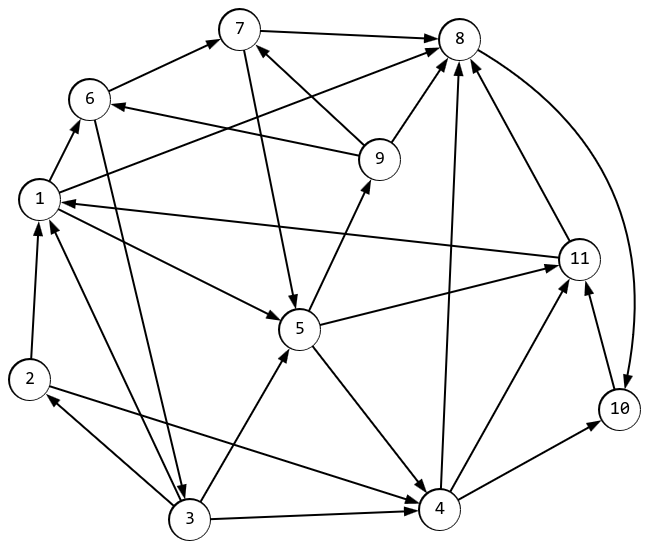
\includegraphics[scale=0.5]{./images/graph5.png}
		\caption{Ориентированный граф}
	\end{figure}
	
	У составленного графа 11 вершин и 26 ребёр, соединяющих их.
	
	\subsection{Составление матрицы и её анализ}
	
	Составим теперь матрицу следующего вида:
	
	$$
	M = \begin{bmatrix}
		m_{11} & m_{12} & \cdots & m_{1n} \\
		m_{21} & m_{22} & \cdots & m_{2n} \\
		m_{11} & m_{12} & \cdots & m_{1n} \\
		\vdots & \vdots & \ddots & \vdots \\
		m_{n1} & m_{n2} & \cdots & m_{nn} \\
	\end{bmatrix}
	,
	$$
	где $m_{ij}=\frac{\text{число стрелок, выходящих из }j \text{-й вершины и входящих в } i \text{-ую вершину}}{\text{общее число стрелок, выходящих из }j \text{-ой вершины}}$
	
	\vspace{3mm}
	
	Итак, получаем следующую матрицу:
	
	$$
	M = \begin{bsmallmatrix}
0 & 0.5 & 0.25 & 0    & 0    & 0   & 0   & 0 & 0    & 0 & 0.5 \\
0 & 0 	& 0.25 & 0    & 0    & 0   & 0   & 0 & 0    & 0 & 0 \\
0 & 0 	& 0    & 0 	  & 0    & 0.5 & 0   & 0 & 0    & 0 & 0 \\
0 & 0.5 & 0.25 & 0 	  & 0.33 & 0   & 0   & 0 & 0    & 0 & 0\\
0 & 0 	& 0.25 & 0    & 0    & 0   & 0.5 & 0 & 0    & 0 & 0\\
0 & 0 	& 0    & 0    & 0    & 0   & 0   & 0 & 0.33 & 0 & 0\\
0 & 0 	& 0    & 0    & 0    & 0.5 & 0   & 0 & 0.33 & 0 & 0 \\
1 & 0 	& 0    & 0.33 & 0    & 0   & 0.5 & 0 & 0.33 & 0 & 0.5\\
0 & 0 	& 0    & 0    & 0.33 & 0   & 0   & 0 & 0    & 0 & 0\\
0 & 0 	& 0    & 0.33 & 0    & 0   & 0   & 1 & 0    & 0 & 0\\
0 & 0 	& 0    & 0.33 & 0.33 & 0   & 0   & 0 & 0    & 1 & 0
	\end{bsmallmatrix}
	$$
	
	Произведем сингулярное разложение и найдём собственный вектор, соответствующий наибольшему собственному числу:
	$$
	v_{max} = \begin{bmatrix}
		0.28 \\
		0 \\
		0 \\ 
		0 \\
		0 \\
		0 \\
		0 \\
		0.55 \\
		0 \\
		0.55 \\
		0.55\\
	\end{bmatrix}, \lambda_{max}=1
	$$
	
	\subsection{Ранжировка}
	Переключимся с Matlab на Python (потому что все примеры в статьях с pagerank приведены на Python, а ещё потому что мне не хочется активно пользоваться функциями в Matlab'e - они там странные :)). Используем следующий код для провередния ранжировки страниц:
	\begin{lstlisting}
import numpy as np

def pagerank(A, k):
	n = A.shape[1]
	v = np.ones(n) / n
	for i in range(k):
		v = A.dot(v)
	return v

A = [[0, 0.5, 0.25, 0,     0,    0,    0,    0,  0,    0, 0.5],
	[0,  0,   0.25, 0,     0,    0,    0,    0,  0,    0, 0],
	[0,  0,   0,    0,     0,    0.5,  0,    0,  0,    0, 0],
	[0,  0.5, 0.25, 0,     1/3,  0,    0,    0,  0,    0, 0],
	[0,  0,   0.25, 0,     0,    0,    0.5,  0,  0,    0, 0],
	[0,  0,   0,    0,     0,    0,    0,    0,  0.33, 0, 0],
	[0,  0,   0,    0,     0,    0.5,  0,    0,  0.33, 0, 0],
	[1,  0,   0,    1/3,   0,    0,    0.5,  0,  0.33, 0, 0.5],
	[0,  0,   0,    0,     1/3,  0,    0,    0,  0,    0, 0],
	[0,  0,   0,    1/3,   0,    0,    0,    1,  0,    0, 0],
	[0,  0,   0,    1/3,   1/3,  0,    0,    0,  0,    1, 0]]
A = np.array(A)
v = pagerank(A, 100)

for i in range(len(v)):
	print(f"{i+1}: {round(v[i], 3)}")
		
	\end{lstlisting}
	
	Здесь матрица A равна M из пункта выше. Мы не говорили, но по элементы $m_{ij}$, из которых составлена эта матрица, по своей сути означают вероятность попадания из $j$ страницы в $i$ при учёте, что наш пользователь никак не опирается на прочие факторы страницы $i$ (таких как ссылка и прочее - не думаю, что кто-то захотел перейти на сайт с названием lolka.ru).
	
	Итак, алгоритм pagerank полностью основан на марковских процессах. Изначально мы можем попасть на любую из $j$ страниц с равной вероятностью (её задаёт отнормированный вектор v), после мы $k$ число раз умножаемся на A (марковские процессы в силе) и получаем результирующий вектор вероятности попадания на ту или иную страницу \textit{в целом} - звучит круто!
	
	Вот результат работы для нашей матрицы $A=M$ (были убраны числа, так как слева и так идёт нумерация):
	\begin{lstlisting}
0.143
0.0
0.0
0.0
0.0
0.0
0.0
0.285
0.0
0.285
0.285		
	\end{lstlisting}
	
	Кстати, если вспомнить собственный вектор $v_{max}$, соответствующий максимальному собственному числу, то он показал те же условно <<важные>> страницы, причем он также учёл распределение вероятностей - у 8, 10 и 11 они наибольшие и одинаковые, а вот у 1 она чуть поменьше. Оно и понятно, ведь в марковских процессах в итоге берут вверх самые большие!
	
	Стоит также отметить, что в алгоритме мы не учитывали параметр затухания $d$, который так же играет важную роль, - в реальном мире при переходе от страницы к странице мы основываемся не только на наличии ссылки, но и её сути!
	
	\textbf{На этом всё, спасибо!}
	
\end{document}
